% Koma-Script Basisklasse
\documentclass[a4paper,12pt,pagesize,headsepline,bibtotoc,titlepage]{scrartcl}

\usepackage[english]{babel}
\usepackage[utf8]{inputenc}     % direkte Eingabe von Umlauten & Co. (Vorsicht: Encoding im Editor muss auch UTF-8 sein!)

\usepackage[T1]{fontenc}            % T1-Schriften

\usepackage{mathptmx}           % Times/Mathe \rmdefault
\usepackage[scaled=.90]{helvet} % Skalierte Helvetica \sfdefault
\usepackage{courier}            % Courier \ttdefault

% Zusatzpakete für mehr mathematische Symbole, Einfügen von Grafiken
% und bessere Bildunterschriften
\usepackage{amsmath,amsthm,amsfonts,graphicx,caption}

% Wenn man direkt mit dem pdflatex eine PDF-Datei erzeugt, sollten diese beiden Pakete eingebunden werden
\usepackage{hyperref} % Hyperlinks anklickbar
\usepackage{ae,aecompl} % bessere Bildschirmschriftarten usw.
\usepackage{cite}
\usepackage{listings}
\usepackage{float}

\usepackage[dvipsnames]{xcolor}
\usepackage{textcomp}
\lstdefinelanguage{XML}
{
  basicstyle=\ttfamily\footnotesize,
  morestring=[b]",
  moredelim=[s][\bfseries\color{Maroon}]{<}{\ },
  moredelim=[s][\bfseries\color{Maroon}]{</}{>},
  moredelim=[l][\bfseries\color{Maroon}]{/>},
  moredelim=[l][\bfseries\color{Maroon}]{>},
  morecomment=[s]{<?}{?>},
  morecomment=[s]{<!--}{-->},
  commentstyle=\color{DarkOliveGreen},
  stringstyle=\color{blue},
  identifierstyle=\color{red}
}
\lstdefinelanguage{Java}
{
  showspaces=false,
  showtabs=false,
  breaklines=true,
  showstringspaces=false,
  breakatwhitespace=true,
  commentstyle=\color{pgreen},
  keywordstyle=\color{pblue},
  stringstyle=\color{pred},
  basicstyle=\ttfamily,
  moredelim=[il][\textcolor{pgrey}]{$$},
  moredelim=[is][\textcolor{pgrey}]{\%\%}{\%\%}
}

\pagestyle{headings}

% Abstand der Kopfzeile vom Text:
\headsep4mm

\typearea[current]{current}     % Satzspiegel neu berechnen

% andere Bildunterschrift mit Hilfe von caption
\renewcommand{\figurename}{Abb.}
\renewcommand{\captionlabelfont}{\bf}

\title{
    \includegraphics*[width=0.4\textwidth]{hpi_logo.png}\\
    \vspace{24pt}
    Recognizing Famous Places on Android
}
\subtitle{
    Seminar\\
    Practical Applications of Multimedia Retrieval\\
    Winter Semester 2016/2017
}
\author{
    Tim Oesterreich, Romain Granger\\[12pt]
    Supervisors:\\
    Haojin Yang, Christian Bartz\\
    Prof. Dr. Christoph Meinel
}
\date{\today}

\begin{document}
\lstset{language=Java}
\maketitle
\tableofcontents
\newpage

\section{Introduction}
As deep learning is becoming an increasingly big influence in everyday applications, more and more focus is put into increasing its distribution to different platforms. During the winter semester 2016/2017 a project seminar emerged, that laid focus on developing a mobile phone application for Google's Android operating system that is capable of recognizing famous sights in big cities from images taken with a smartphone camera.\\
Modern smartphones can in some cases outperform mid-range notebooks from a couple of years ago and, most interestingly, often have a dedicated GPU\footnote{Graphics Processing Unit}. GPUs are usually used for deep learning because of their high parallelization capabilities.\\
Part of this seminar was the evaluation of a fairly recent deep learning framework called CNNDroid \cite{cnndroid2016}, which uses GPU acceleration for classification and promises substantial performance improvements compared to CPU classification.
\section{CNNDroid}
CNNDroid is an open source deep learning library for Android. It is able to execute convolutional neural networks, supporting most CNN layers used by existing desktop/server deep learning frameworks, namely Caffe, Theano and Torch. Supported layers, as of March 2017 are:
\begin{itemize}
    \item{Convolutional Layer}
    \item{Pooling Layer}
    \item{Local Response Normalization Layer}
    \item{Fully-Connected Layer}
    \item{Rectified Linear Unit Layer (ReLU)}
    \item{Softmax Layer}
    \item{Accuracy and Top-K Layer}
\end{itemize}
Due to the library being open source, it is possible to add additional layers, such as batch normalization or sigmoid.\\
The library also supports a variety of customizations, like maximum memory usage, GPU or CPU acceleration and automatic performance tuning.

\subsection{Setup and Integration into Android Project}
CNNDroid is a source code library. That means that integration into an existing Android Project is fairly straight forward and doesn't require any third-party dependencies.\\
The only prerequisites are:
\begin{itemize}
    \item{A functional Android development environment (e.g. Android Studio\footnote{https://developer.android.com/studio/index.html})}
    \item{Android phone or emulator running at least Android SDK version 21.0 (Lollipop)}
\end{itemize}

To integrate CNNDroid into the project, the repository has to be cloned from its GitHub\footnote{https://github.com/ENCP/CNNdroid} page. Inside the \texttt{CNNdroid Source Package}' folder are three folders: \texttt{java}, \texttt{rs} and \texttt{libs}.\\
The \texttt{java} and \texttt{rs} folders need to be copied into the projects \texttt{app/src/main/} directory, merging the \texttt{java} folders.\\
The \texttt{libs} folder has to be copied and merged into the \texttt{app/} directory.\\
For effective usage of CNNDroid, it needs read and write access to storage on the smartphone. Android policies require an application to request these permissions before the app starts. These permission requests are specified inside the \texttt{AndroidManifest.xml} file. The following lines have to be added there before the \lstinline[language=XML]{<application} section:

\begin{lstlisting}[language=XML, basicstyle=\scriptsize]
    <uses-permission android:name="android.permission.READ_EXTERNAL_STORAGE"/>
    <uses-permission android:name="android.permission.WRITE_EXTERNAL_STORAGE"/>
\end{lstlisting}

To cope with the high computational requirements, CNNDroid potentially needs a large amount of memory. Therefore, the heap has to be increased, which is done by adding

\begin{lstlisting}[language=XML, basicstyle=\scriptsize]
    android::largeHeap="true"
\end{lstlisting}
\noindent
inside the \lstinline[language=XML]{<application} section.\\
Now, everything should be set up correctly and programming can commence.\\
After importing the package \lstinline[language=Java]{network.CNNdroid}, the \lstinline[language=Java]{CNNdroid} object is accessible, which can call the function \lstinline[language=Java]{CNNDroid::classify}. This is the keyword to start execution of the trained model. The specification of the model is explained in the following section.

\subsection{Structure of necessary CNNDroid Files}
Of course, CNNDroid needs to know how to classify an input. For that it either uses converted binary layer files, created by a desktop deep learning framework, or internal conversion functions (e.g. for pooling or ReLU).\\
The layer BLObs\footnote{Binary Large Objects} are generally used for more complicated layers, such as convolutional or fully connected layers, which have high dimensional variables (weight matrices). These files have to be converted into the MessagePack\footnote{http://msgpack.org/} format and put onto the smartphones storage.\\
The order in which the layers are executed, additional configurations and layers which do not need a BLOb file are defined inside the definition file. This file is used as a settings file for the \lstinline[language=Java]{CNNdroid} classifier.\\
On creation of the \lstinline[language=Java]{CNNdroid} object, the absolute path to this file has to be specified.\\
Configurations, other than the layer definitions are:
\begin{itemize}
    \item{the absolute path to the layer blob files\\(\lstinline[language=Java]{root_directory: "/absolute/path/to/layer/files"})}
    \item{the maximum amount of RAM the classifier should use on the smartphone\\(\lstinline[language=Java]{allocated_ram: Amount_in_MB})}
    \item{whether or not automatic performance tuning should be used\\(\lstinline[language=Java]{auto_tuning: "on|off"})}
    \item{whether or not classification should be GPU accelerated (if possible)\\(\lstinline[language=Java]{execution_mode: "sequential|parallel"})}
\end{itemize}
Layers are defined as shown in figure \ref{fig:def_file}.

\begin{figure}[H]
  \centering
    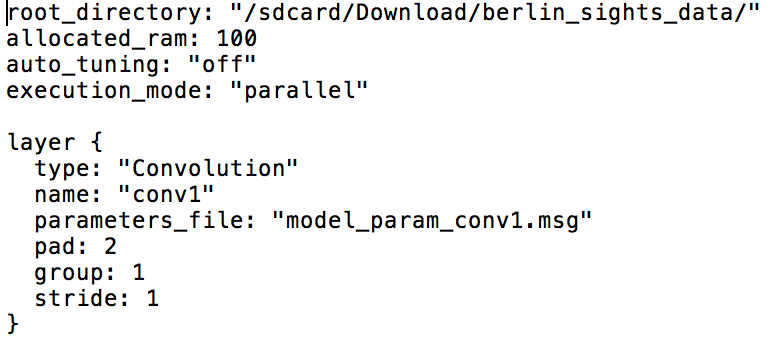
\includegraphics[width=0.5\textwidth]{def_file.png}
  \caption{Excerpt of a CNNDroid definition file}
  \label{fig:def_file}
\end{figure}

Not essential for the execution of CNNDroid, but very helpful for processing the final results, is a labels file. This file should specify human-readable names for the extractable classes. The order inside this file should be mapped to the output order of the last layer (probably a fully-connected layer), i.e. the first value of the output array should correspond to the first class name inside the labels file. The class names should be newline-separated.

\subsection{Training the model}
We trained our deep learning model based on crawled images with the caffe framework. The training occurred on an HPI server (accessible under the IP 172.16.18.178 and username msws2016t1). Caffe is already installed there and a variety of crawled images, as well as a labels file with the paths to each image are available inside the \texttt{training\_data} folder. Inside the same folder you can also find the \texttt{training\_full.sh} script, which can be executed to start the training and create a model.\\
An example model can be found in the \texttt{training\_data/berlin\_sights\_model} folder.\\
In order to test the model quickly, caffe provides an ipython notebook on their Github repository. This repository is checked out in the \texttt{caffe} folder. To start the notebook an ssh-tunnel has to be created to your local machine, e.g. using\\\\
\texttt{ssh -N -f -L localhost:8888:localhost:8889 msws2016t1@172.16.18.178}\\\\
Using a normal ssh connection to the server, the notebook can be executed with the command\\\\
\texttt{ipython notebook --no-browser --port=8889}\\\\
and viewed in a webbrowser on the local machine under the address \texttt{localhost:8888}.\\
The notebook itself provides possibilities to classify an image downloaded from a web address, view the output of specific layers and more.

\subsection{Convert Trained Models into CNNDroid-compatible Format}
As mentioned before, CNNDroid uses a format called MessagePack for the layer definitions. MessagePack is a binary serialization format for exchanging data, comparable to JSON\footnote{JavaScript Object Notation}, but other than JSON it is not human-readable. The omission of this constraint makes it possible to reduce size and increase parsing speed of the data stored inside. This is especially important due to the limited storage that most smartphones posses, especially compared to big servers, where deep learning is usually executed.\\
Figure \ref{fig:json_vs_msgpack} illustrates how MessagePack saves storage space by using types (JSON encodes everything as strings, so for example, `true' uses four Bytes, while it only uses one Byte using MessagePack) and dropping control symbols, like the curly braces \{\}.

\begin{figure}[H]
  \centering
    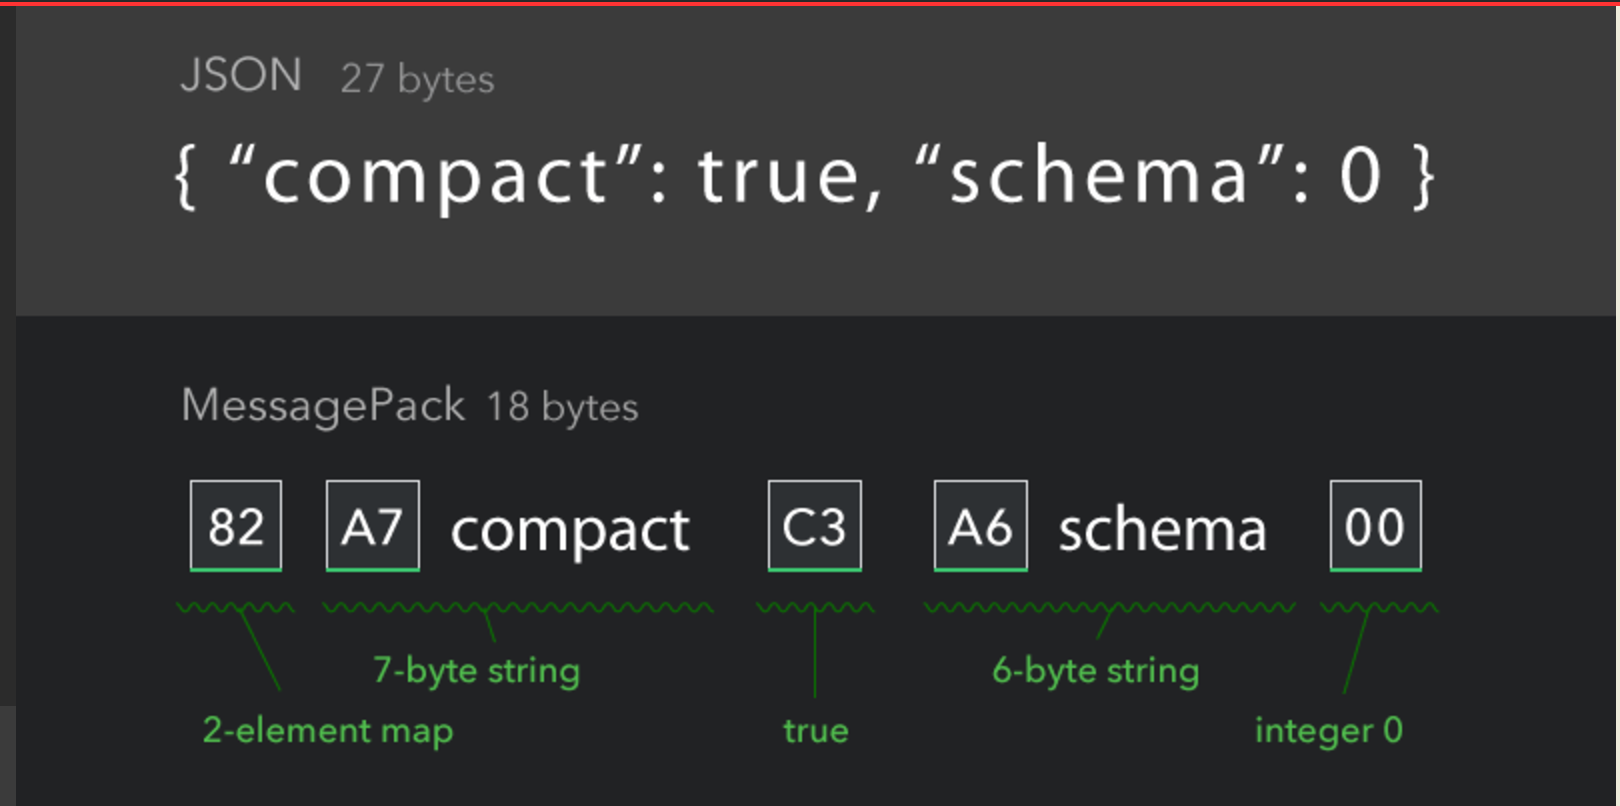
\includegraphics[width=0.5\textwidth]{json_vs_msgpack.png}
  \caption{Comparison JSON and MsgPack}
  \label{fig:json_vs_msgpack}
\end{figure}

In order to convert models from the aforementioned desktop/server deep learning frameworks, CNNDroid provides conversion scripts, which can be found in the\\
\texttt{CNNDroid/Parameter Generation Scripts/} folder. The script for Caffe is written in Python and requires the packages \lstinline[language=python]{numpy} and \lstinline[language=python]{msgpack} to be installed.\\
Three variables need to be defined inside the script.
\begin{itemize}
  \item{\texttt{MODEL\_FILE} - The absolute path to the trained model}
  \item{\texttt{MODEL\_NET} - The absolute path the deployment prototxt file, which specifies the parameters for the layers}
  \item{\texttt{SAVE\_TO} - The saving path}
\end{itemize}
The output are converted layer files in MessagePack format. The definition and label files have to be created manually. For the definition file, most of the content of the prototxt deployment file can be used. Only some parts of the syntax have to be adapted to a CNNDroid parsable format.\\
\newpage
\subsection{CPU vs GPU performance}
For a comparison of the sequential and parallel mode of CNNDroid we used the Android emulator using 2 GB of RAM. We used the berlin sights classifier, provided in the berlin\_sights\_data folder.

\begin{center}
  \begin{tabular}{l|c|r}
    layer & sequential time in ms & parallel time in ms \\\hline
    conv1 & 277 & 75\\
    pool1 & 22 & 47\\
    relu1 & 1 & 1\\
    conv2 & 299 & 27\\
    pool2 & 8 & 23\\
    conv3 & 161 & 24\\
    pool3 & 4 & 6\\
    ip1 & 1 & 5\\
    ip2 & 0 & 0\\
    prob & 0 & 0\\\hline
    sum & 773 & 208\\
  \end{tabular}
\end{center}

We can see that especially the more complicated convolutional layers profit from the additional speed of the GPU. Copying data from the RAM to GPU memory is usually very high, which is why the sequential mode can be faster for layers that do not do a lot of processing. In general, the parallel, GPU-accelerated processing speed is about three times faster than sequential, CPU-only processing.\\
The CNNDroid paper\cite{cnndroid2016} states a 12-times speedup with the CIFAR10 dataset on a Samsung Galaxy Note 4.\\
Our test machine was a MacBook Pro with an Intel Iris Graphics 6100 GPU and a 2.9 GHz Intel Core i5 CPU using the Android Studio emulator.\\
Apparently, the emulator does not reach such a significant overall speedup as the one stated in the paper. The \texttt{conv2} layer reaches an 11-times speedup, which comes close, but in sum it only reaches a third of the expected performance.\\
This however can potentially have a variety of reasons. Our testing setup does not follow lab conditions. It is not possible to know how the Android Studio emulator uses the MacBooks resources. Additional overhead is to be expected when communicating with the hardware. Also the CPU in the MacBook is more powerful than the one inside the Samsung phone (using an NVidia Jetson-style dual CPU consisting of one Quad-core 1.9 GHz Cortex-A57 and one Quad-core 1.3 GHz Cortex-A53, usually only using the A57 for high-computation tasks), which would decrease the speedup for the parallelized computation as the sequential computation is faster.\\
In theory the GPU of the MacBook should perform a lot better than the Samsung Galaxys GPU (which is capable of 48 parallel tasks, while the MacBooks GPU is capable of many hundred computations at the same time), it is however possible that the layer doesn't provide so many calculations, so that the full performance can not be used.\\
Overall, it is apparent, that the parallelization of the classification creates a clear speedup, which does however not reach that promised in the paper using our test setup.
\section{Image Crawler}
Classification of real-world images requires a very big dataset for the learning process beforehand. Google Streetview provides 360 degree images from many places in all German urban areas. Using sophisticated crawling techniques, a huge amount of image data can be extracted from these, so called, `Photospheres'.\\
This chapter describes how we used the Google Streetview and other image APIs to crawl images from famous sights in Berlin.

\subsection{Image Crawler}
We provide a Google Streetview image crawling python script inside the\\\texttt{ImageCrawler/streetview_crawler} folder. This script takes a CSV\footnote{Comma-Separated Values} file as input, which specifies the parameters the crawler needs, such as position and viewing angle. Chapter \ref{csv_file} explains the contents of this file.\\
All requirements for the crawler are specified in the \texttt{requirements.txt} file and can be installed with the command \texttt{\$ pip install -r requirements.txt}.\\
Given a location in longitude and latitude, the image crawler will automatically create jpeg-images from different viewing angles. These angles can either be specified or automatically generated by calculating the angle between two geo-coordinates. In the latter case, the script will generate images in five degree steps from 30 degrees to the left to 30 degrees to the right of the calculated viewing angle. If specified by hand, we use one degree steps from the starting to the end angle.\\
Because photospheres can change or get removed, the API uses the closest photosphere to the location provided. This might not be the location specified in the CSV file, which is why we also check the metainformation of each photosphere for the coordinates connected to the image and the status code. In case there is no image in a certain area, the status code tells us that and we don't need to go through all the requests.\\
To prevent Denial-of-Service attacks, the API uses a time- and request-based blocking system. That means, that an IP might be denied further downloads if it either makes request too fast or it reaches the maximum amount. To counter the first blockage, our script uses an exponential wait mechanism. If requests were made too quickly, it waits for a short while before retrying. If it still gets no result, the wait time is increased. This is repeated until the blockage is lifted.\\
For the second part, we provide the usage of a Google API key\footnote{https://developers.google.com/maps/documentation/streetview/}, which can be passed to the crawler script with the \texttt{---key \{key\}} command line switch. The API key enables the crawler to request up to 25'000 requests per day for free, with the option to increase the volume against money.

\subsection{Setup of viewing parameters}\label{csv_file}
Inside the \texttt{places.csv} file, the crawler finds parameters for specified locations and their photospheres.\\
The necessary fields are:
\begin{itemize}
    \item{lat - the latitude of the photosphere in decimal format}
    \item{long - the longitude of the photosphere in decimal format}
    \item{fov - the field-of-view of the photosphere section in degrees}
    \item{pitch - the pitch of the camera in degrees (0 degrees equals parallel to the floor)}
    \item{starthead - the heading from where the camera sweep should start, or 0 if heading should be calculated automatically [optional, if buildingLat and buildingLong specified]}
    \item{endhead - the heading where the camera sweep should end, or 0 if heading should be calculated automatically [optional, if buildingLat and buildingLong specified]}
    \item{name - the name of object in the image; this name is being used as a file prefix for easier identification}
    \item{buildingLat - the latitude of the object in the image; used for automatic heading calculation [optional, if starthead and endhead specified]}
    \item{buildingLong - the longitude of the object in the image; used for automatic heading calculation [optional, if starthead and endhead specified]}
\end{itemize}

The values are read line-by-line and have to be comma-separated.

\subsection{State of Automation}
The static image API we use only provides data about one specific photosphere. This enables us to get a fair amount of images from different viewing angles and different zoom levels for each position specified.\\
As mentioned before, we currently do a camera sweep from a start heading to an end heading, taking one image per degree. This creates on average 40 different viable images. Additionally, we scale each crawled image to 90\% and 80\% of its size, so we gain about 120 images for each line in the CSV file.\\
Unfortunately, this API doesn't provide the possibility to find out which further photospheres are nearby. For example, it is not possible to ``drive down'' a road by pressing the arrows, like on the Google Maps website.\\\\
As a future improvement, the JavaScript API could be used to find out which locations provide images and use this information to crawl more data with less manual work.\\
Also, to improve the quality of the images, it is possible to classify each image with our own sights classifier and find out if the object we search is actually in it and the image is not corrupted by other objects that we might also want to classify.

\subsection{Current Limitations}
Complete automation is not consistently possible at the moment. The static Image API we use for downloading the images does not work on the same database as the JavaScript API, that Google Maps uses. Therefore it is not easily possible to download many of the photospheres from the Streetview web service and results for the same geo-coordinates usually differ between the Image and the JavaScript API. There is currently a feature request open to resolve this issue\footnote{https://code.google.com/p/gmaps-api-issues/issues/detail?id=10402\&q=apitype\%3AStreetView\&sort=-stars\&colspec=ID\%20Type\%20Status\%20Summary\%20Internal\%20Stars}.\\
Another limitation is the reported geo-coordinates in the metadata of the photospheres. These coordinates are usually provided by the camera that took them. GPS can be inaccurate up to 30-40 meters in bad cases. Especially if the image was taken very close to the object, this deviation can cause the automatic calculation of the heading to be wrong and not contain the object observed. This is why the CSV-file also provides the possibility to specify the starting and end heading.

\subsection{Google Places API}
For our project, we use several APIs from Google which help us to get additional information about places. Mainly, this is complementary information such as: Name and address of the place, phone number, website and rating from Google reviews.

\subsubsection{Place Detection API}
The place detection API allows us to discover places close to where the device is located. These are all places registered in Google including local businesses, points of interest, and geographic locations. This API will return a maximum of 10 probable places.
Another very interesting use is that it can help us determinate if our prediction is relevant, by comparing our classification with the results from this function.
\newpage
\subsubsection{How to use it in Android}
The first step is to get an API key from Google\footnote{https://developers.google.com/}. To get the API key, you need to register on the developer console from Google. This platform is used to access every Google API registered by your company.

After that, you need to declare your API key in the android manifest between the \lstinline[language=XML]{<application} tag and the first \lstinline[language=XML]{<Activity>} tag:

\begin{lstlisting}[language=XML, basicstyle=\scriptsize]
<meta-data
android:name="com.google.android.gms.version" android:value="@integer Google_play_services_version"/>
<meta-data
android:name="com.google.android.geo.API_KEY" android:value="API_KEY"/>
\end{lstlisting}

For the third step, you need to ask permissions in the android manifest for Internet access and GPS location.
\begin{lstlisting}[language=XML, basicstyle=\scriptsize]
<uses-permission android:name="android.permission.INTERNET"/>
<uses-permission android:name="android.permission.ACCESS_NETWORK_STATE"/>
<uses-permission android:name="android.permission.ACCESS_FINE_LOCATION"/>
\end{lstlisting}

In your application, you need to declare a "GoogleApiClient" builder and add the APIs you want to use. In our case, and illustrated by the following snippet, we use the \texttt{PLACE\_DETECTION\_API} and \texttt{GEO\_DATA\_API}.

\begin{lstlisting}[language=Java, basicstyle=\scriptsize]
mGoogleApiClient = new GoogleApiClient.Builder(this)
                   .addApi(Places.PLACE_DETECTION_API)
                   .addApi(Places.GEO_DATA_API)
                   .enableAutoManage(this, GOOGLE_API_CLIENT_ID, this)
                   .build()
\end{lstlisting}

The final step is calling the API function. You need to use the \texttt{Places} package associated with the API you want to use. The Google API builder has to be passed to the function.
\begin{lstlisting}[language=Java, basicstyle=\scriptsize]
#For the PLACE DETECTION API
Places.PlaceDetectionApi.getCurrentPlace(mGoogleApiClient, null);

#For the GEO DATA API
Places.GeoDataApi.getPlaceById(mGoogleApiClient, placeId)
\end{lstlisting}

\subsubsection{Limitations}
Google provides a really useful and powerful service, but the requests are very limited. We can only have 1'000 free requests per 24 hours, which is probably not enough enough for a multi-user application.
Therefore, Google provides a business API plan that can be adapted if needed. It gives access to 150'000 request per day and can be increased depending on the number of requests needed.

\subsection{Shutterstock, Flickr and Pinterest}
Shutterstock\footnote{https://www.shutterstock.com/}, Flickr\footnote{https://www.flickr.com/} and Pinterest\footnote{https://www.pinterest.com/} are public web application for hosting and sharing photos and images. For example, on Flickr nearly 7,000 photos are uploaded per minute.
As these services are used by both professional and amateur photographers, we can find a lot of good quality images.

\subsubsection{Example to get images URL}
This is an example about how to get an image URL which can be downloaded, using the angularJS API package and store the resulting image in a mongoDB database.\\
First we create an API object:
\begin{lstlisting}[language=Java, basicstyle=\scriptsize]
var api = shutter.v2({
    clientId: 'Your public key',
    clientSecret: 'Your secret key',
});
\end{lstlisting}

Then we detail the search string we want to crawl. Here we choose the Brandenburg Gate.

\begin{lstlisting}[language=Java, basicstyle=\scriptsize]
var opts = {
    query: 'Brandenburg Gate',
    page: 1,
    per_page: 200,
    sort : 'popular'
};
\end{lstlisting}

Finally, we navigate through the JSON response to get the URL.

\begin{lstlisting}[language=Java, basicstyle=\scriptsize]
    api.image.search(opts, function(err, data) {
        if (err) throw err;

        console.log(data.data[0].id);
        var arrayLength = data.data.length;

        for (var i = 0; i < arrayLength; i++) {
            var obj = data.data[i];
            console.log(obj);
        }
\end{lstlisting}
\newpage
The response return will be as follows.\\
\\
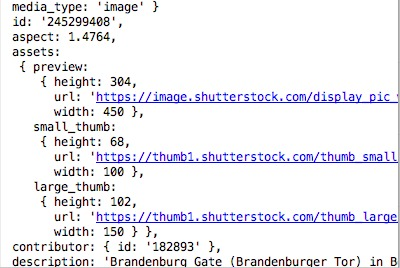
\includegraphics{jsonShutter}

\subsubsection{Limitations}
These services are limited to 3600 call per hours. An API key can be blocked if the service detects an abusive use of the service.

\section {PlaceRecognizer Application}
Overview: What does it do. Whom is it for. How does it achieve its task?

\subsection {CNNDroid Integration/Image Classifier}
Explain ImageClassifier Class; Including Variables that need adaption when changing Layers or DataSets\\
How to put msgpack on phone

\subsection {Real-Time Frame Capture}
How does the camera talk to the Image Classifier?

\subsection {GPS Logger}
How do we get GPS values and how can we integrate them?

\subsection {Wikipedia Parser}
How do we get the text for a classified image from Wikipedia?

\subsection{How to setup project in Android Studio}
\section{Outlook}
We have several ideas to improve our application.\\

Right now the application is very basic. It only contains two buttons which call the most essential functions and show the most essential information. Improvements of the visualization, like showing the camera image in full screen and switching to the information pane on getting a result, providing an option page, for example for switching language or user or possibilities to receive further information about a recognized place by showing links to Wikipedia or Google could add a lot of user experience to the application.\\
Because our application is aimed at international tourists, it is a good idea to localize it. This can be achieved by providing translation resource files, which cold look like this:
\begin{lstlisting}[language=XML, basicstyle=\scriptsize]
    #/values/strings.xml:
    <resources>
        <string name="hello_world">Hello World!</string>
    </resources>
\end{lstlisting}

\begin{lstlisting}[language=XML, basicstyle=\scriptsize]
    #/values-es/strings.xml
    <resources>
        <string name="hello_world">iHola Mundo!</string>
    </resources>
\end{lstlisting}

Also for the Wikipedia parser, we can get the phone language with a simple line of code
\begin{lstlisting}
    Locale.getDefault().getDisplayLanguage();
\end{lstlisting}

Lastly, a naive solution for improving the recognition results, especially if many objects are nearby is pre-filtering the possible results using the current position and only allowing results that are within a certain radius. A more complex approach would be to include the coordinates into the training itself. That means that a result is not only based on computing pixel values, but also considers the current position. This would provide an additional degree of confidence into the calculated result.\\

\begin{figure}[hbp]
\begin{center}
\includegraphics*[width=0.75\textwidth]{beispiel.png}\\
\caption{Eine Abbildung, Quelle: \cite{cnndroid2016}}
\label{abb:test}
\end{center}
\end{figure}

\newpage
\bibliography{bibliography}{}
\bibliographystyle{plain}

\end{document}